\documentclass{article}
\usepackage{relsize}
\usepackage{lmodern}
\usepackage{textcomp}
\usepackage{graphicx}
\usepackage{hyperref}
\usepackage[utf8]{inputenc}

\title{The truth about chatbots \\[0.4em]\smaller{}Session n\,°2: Chatbot design}
\author{Louise Crépet}
\date{March 2019}

\begin{document}

\maketitle

\textit{Special thanks to Marine Froment, Marie Feld and Célia Corsin for sharing their work and answer to my questions!}

\newpage
\section{Introduction}
A chatbot methodology has been designed by product owners and designers from Fabernovel Technologies Applidium (FTA), with a little help from the developers. It’s used to conceive and develop chatbots for customers and internal needs.
More specifically, it helped to develop a “QuizBot” on Slack, as an internal project at FTA.

\section{Understand}
“Understand” is the first step of the chatbot conception. We must understand the business and human needs, the expectations and the brand. We also have to define the target: who are the future users?
Questions to ask:
\begin{enumerate}
    \item On which channel(s) the chatbot will be available? Usually, you have data about the customers/potential users, so you know the contacts points.
    \item Do you need administration? Sometimes, you want to administrate resources used by the chatbot, manage the users for example, create documents…
    \item Do you need human intervention? When the chatbot cannot answer, does it hand over to a human? Through what channel?
    \item Do you want Natural Language Processing (NLP)? Does the chatbot understand inputs written by the users or only commands?
    \item What are the available languages? Should the chatbot speak only french or english, or is it multilingual?
    \item What are the analytics? Which data about your chatbot and its usage do you want to record?
    \item Do you want to handle non-response? Should the chatbot repeat its last question or just give up?
\end{enumerate}
And don’t forget the GDPR! The chatbots sometimes have to save private data about users, like email address or phone number.\\
\break 
How did we start with the QuizBot?\\ In the context of the internal training, we want to test the knowledge of the staff: what have they retained just after the formation? a few months after?\\
Why not use a chatbot? We already have a channel: Slack is used everyday by everyone.
For now, we all speak french, but we keep in mind that will maybe change. No human intervention is needed, but we’ll need an administration console to create the quizzes, the questions and the answers. And we can use a bit of NLP!

\section{Storyboard}
The second step will require a white board and a marker: we are going to draw all the typical scenarios for each type of question the chatbot can handle. We need to define the typical flow: 
\begin{itemize}
    \item What’s the hook? 
    \item How does the bot say goodbye at the end? 
    \item What does it say when it doesn’t understand or cannot answer? The errors are particularly important: the chatbot will fail and it should handle the failures.
    \item How does it react when the user doesn’t talk anymore?
    \item Does the chatbot need to access data from external systems? When? Are these external systems already available?
    \item When should the analytics be recorded?
    \item If the chatbot can hand over to a human, how is the transition made?
\end{itemize}


An interesting thing to do is to test your scenarios on real people and potential users. You can use an instant messaging app and real persons can play the role of the chatbot; they just have to follow scrupulously the flow of the chatbot. This way, you can validate or invalidate a complete scenario or a part of it.\\
\break
Let’s take a typical QuizBot's flow: 
\begin{enumerate}
    \item Alice asks the chatbot to send a quiz to Bob
    \item Bob answers to all the questions of the quiz
    \item the chatbot posts Bob’s results
\end{enumerate}


The chatbot understands the requests, but uses buttons to propose answers to users during the quiz.\\
\break
At the end, we obtain this diagram:\\
\break
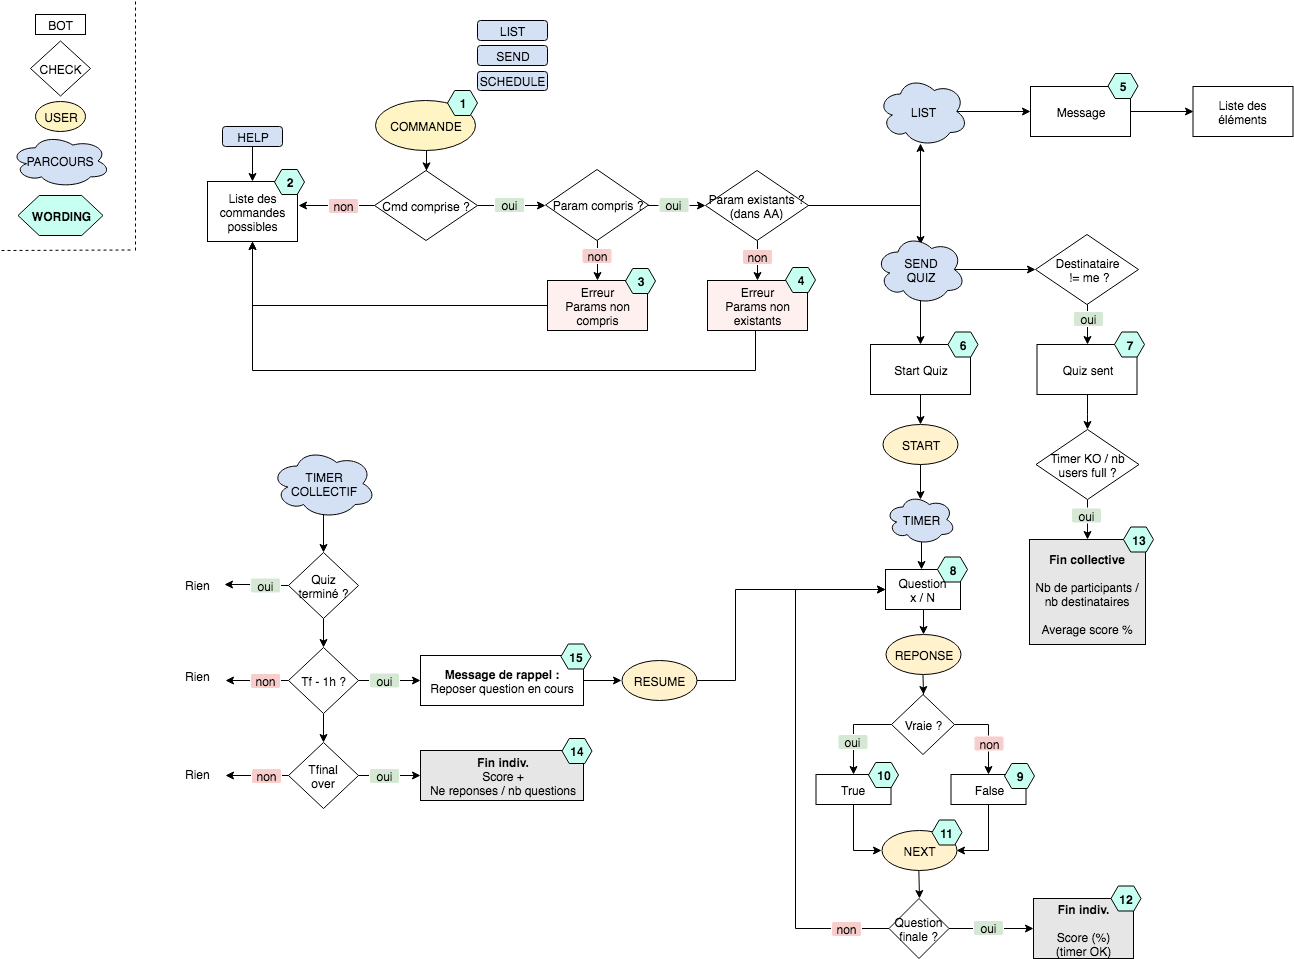
\includegraphics[scale=0.3]{images/quizbot_graph.png}

\newpage
\section{Personality}
The fun part is coming: personality! We are going to define what’s the attitude, the tone of the chatbot: what image do you want to show through this chatbot? For this step, you can use inspirational bots to find ideas: 
\begin{description}
    \item \textbf{The buddy}: very informal, it's funny, makes jokes and uses a lot of emojis.
    \item \textbf{The nice robot}: it's clearly a little robot and it wants to help. It's happy and informal, but nice and polite.
    \item \textbf{The utilitarian bot}: it uses no emoji, it's not too informal. It has a function and fulfills it.
    \item \textbf{The butler}: it's formal and very polite. Its job is to help you and it takes it seriously.
\end{description}
Of course, this list is not exhaustive!\\
At the end, you’ll have the profile of the chatbot: 
\begin{itemize}
    \item name
    \item graphical representation: picture, graphic guidelines 
    \item “gender”: this includes male/female/non-binary/undetermined, but also animal, robot, alien...
    \item age (if relevant)
    \item goal
\end{itemize}
You'll have determined some characteristics linked to its personality as well: 
\begin{itemize}
    \item tone: formal or not
    \item expression: typical sentences, using emojis or not
    \item general mood: neutral, happy, expressive, nonchalant
\end{itemize} 
And you'll have some typical sentences:
\begin{itemize}
    \item first contact and presentation
    \item presentation of available actions
    \item incomprehension
    \item reaction to non-response, reformulation
    \item end of conversation
\end{itemize}
\break
For the QuizBot, we want a character embodying the knowledge but reassuring at the same time: it’s here to welcome the newbies and help them in their new adventure. At FTA, we also have a kind of tradition: all our bots refer to our common cultural universe. We have Marie-Ange (from the TV show “Qui est qui ?”) to make the newcomers meet their colleagues and Cyril (Lignac) to make the people eat together.\\
The QuizBot will be “Jamy”, like the presenter of the scientific program “C’est pas sorcier” !\\

\includegraphics[scale=0.5]{images/jamy_avatar.png}
\newline
\newline
Jamy speaks french, it uses informal “you” and emojis, and it's fun and expressive.

\newpage
\section{Development}
Now that we have decided what the chatbot does and how it does it, it’s time to implement it. First, the good news: the development of a chatbot is totally compatible with Agile methodologies!\\
Each bot implementation is specific, but here at FTA, we had experimented some design patterns that work well:
\begin{description}
\item \textbf{The state machine}\footnote{\url{https://en.wikipedia.org/wiki/State_pattern}}: allow to keep a “memory” and react according to the context and the previous inputs.
\item \textbf{The chain of responsibility}\footnote{\url{https://en.wikipedia.org/wiki/Chain-of-responsibility_pattern}}: little modules are specialized in answering to one request; if one module cannot answer, it hands over to the next module.
\end{description}

Still at FTA, we have a library that allows to build chatbots: Clarke. One of the advantages is that makes the chatbot “channel agnostic”: you just have to add the corresponding libraries, and Clarke can handle multiple channels (for now, we have implemented the libraries for Messenger and Slack).\\
It’s open-source, you can find it and contribute on Github\footnote{\url{https://github.com/applidium/clarke}}!

\section{Training and tests}
At last but not least: the training and test step.\\
Training is pertinent only if you use NLP: you actually train the NLP engine by giving as much user inputs as you can to improve its understanding. Most of the NLP platforms have an admin console to do that: you can verify if the engine understand correctly what’s it been said.\\
To sum up, the training steps are:
\begin{enumerate}
    \item enrich the NLP engine with expressions, sentences that can be said by users
    \item ask real users to talk to the chatbot: they will certainly use different expressions
    \item correct the engine from the NLP platform if it didn't understand expression, or understood them incorrectly
    \item repeat!
\end{enumerate}
You can train the NLP engine for the whole life of the chatbot.\\
\newpage
The tests allow to validate your final product. You want two things:
\begin{itemize}
    \item Check yourself if the chatbot behaves as expected: is the implementation correct?
    \item Check with users if chatbot works with external people: does it help them? Are the scenarios relevant? Is the chatbot consistent?
\end{itemize}

\section{Checklist}
Ubisend, a chatbot building company, created a “chatbot review checklist”\footnote{\url{https://blog.ubisend.com/hubfs/white-papers/ubisend_chatbot_review_checklist_02.pdf}} that allows to evaluate a chatbot solution, yours or one of your competitors, on some attributes. These attributes are grouped into 6 categories:

\subsection{Branding}
It’s about what the chatbot looks like and what it tells about the company:
\begin{description}
    \item \textbf{Brand consistency}: does it look and feel like the company's chatbot or does it look out of place?
 \item \textbf{Conversational}: is the chatbot appropriately conversational? Does it use small talk, greets, engages?
    \item \textbf{Language consistency}: does the chatbot use language and phrasing that is consistent with the brand's website and image?
\end{description}

\subsection{Performance}
It’s about the chatbot’s job and how well it does it:
\begin{description}
    \item \textbf{Purpose}: is it clear what this chatbot is meant to do? Can you tell what the One True Goal is?
    \item \textbf{Effectiveness}: is it effective at its job? Does it provide the right help?
    \item \textbf{Knowledge}: can it answer common questions around the task it was built to perform? Can it help the user?
    \item \textbf{Feedback}: does it let the user know they are progressing towards their goal?
\end{description}

\subsection{Consistency}
A chatbot should always do its job, and do it well:
\begin{description}
    \item \textbf{Doing its job}: can the chatbot consistently help the user achieve their goal?
    \item \textbf{Journey consistency}: does the path the chatbot takes users fit the expected path the company would take them on?
    \item \textbf{Up to date}: is the chatbot up to date? Is it aware of the latest changes in processes, legalities, etc.?
    \item \textbf{Knowledge}: does the chatbot have a consistent amount of knowledge across the different topics it touches on? Does it know a lot about one thing but nothing about another?
\end{description}

\subsection{Humanity}
It’s about how the chatbot “behaves” with humans:
\begin{description}
    \item \textbf{Transparency}: does it pretend to be a human? Is it transparent and honest about being a machine?
    \item \textbf{Self-aware}: can it answer questions about itself? Does it know and is open about its limitations?
    \item \textbf{Reaching humans}: can it hand conversations over to its human colleagues gracefully? Does it inform the users on how to skip straight to a humans?
\end{description}

\subsection{Affect}
It’s about the chatbot’s “empathy” and appropriateness:
\begin{description}
    \item \textbf{Politeness}: is the chatbot pleasant and polite? Does it treat users with respect? Is it abrupt?
    \item \textbf{Personality}: does the chatbot have a personality? Is it clearly identifiable?
    \item \textbf{Emotions}: does the chatbot convey emotion? Does it appear authentic?
    \item \textbf{Adaptation}: is the chatbot capable of reading the user's mood? Does it adapt to it?
\end{description}

\subsection{Accessibility}
A chatbot is built to be used by most of the users:
\begin{description}
    \item \textbf{Channels}: is the chatbot present on an appropriate channels? Is it accessible across multiple channels?
    \item \textbf{Convenience}: is a chatbot for this particular One True Goal more convenient to the user than another medium or channel?
    \item \textbf{Ease}: is it easy to access and use? Does it understand multiple variations of the same user input, or does it need the user to use specific language or buttons?
    \item \textbf{Context}: does the chatbot remember the context of the conversation, or does it only ever respond to the previous question?
\end{description}

\end{document}
